\newpage
\section{AVALIAÇÃO EXPERIMENTAL}


Para elaboração do modelo de classificação, a partir dos comentários obtidos para o vídeo \textbf{Não Faz Sentido! - Crepúsculo [+13]}, foram escolhidos de forma aletória um grupo de 50\% (32.131) dos comentários para elaboração do modelo de classificação e 50\% (32.130) dos comentários para elaboração do grupo de validação (ou grupo de testes).
Neste Capítulo é descrita toda a execução dos passos mencionados na Figura \ref{fig:metodologia} e no Capítulo 5, utilizando os grupos de comentários para elaboração e validação do modelo.
% Passos sugeridos de acordo com os objetivos específicos:
% Classificar os comentários: (1) Coleta de Dados (2) Pré-Processamento (3) Definição dos Critérios de Classificação
% Analisar os comentários: (4) Treinamento do Modelo de Classificação
% Indicar os vídeos Pejorativos (5) xxxxxx
% Avaliar o modelo de classificação (6) Avaliação do Modelo de Classificação
\subsection{Escolha dos vídeos}
Levando em consideração os critérios de escolha mencionados anteriormente, o tamanho do canal que postou o vídeo e a quantidade de comentários, foram escolhidos os vídeos a seguir:

\begin{itemize}  
    \item \textbf{PARABÉNS DA GALINHA PINTADINHA - Clipe Música Oficial - Galinha Pintadinha DVD 4} \footnote{https://www.youtube.com/watch?v=ei2-RjJDBHc}
	\item \textbf{Galinha Pintadinha 4 - Clipe Música Oficial - Galinha Pintadinha DVD 4} \footnote{https://www.youtube.com/watch?v=gWI4qV2H8VY} 
	\item \textbf{UPA CAVALINHO - Clipe Música Oficial - Galinha Pintadinha DVD 4} \footnote{https://www.youtube.com/watch?v=Fn9adh4HWUU}
	\item \textbf{Pintinho Amarelinho - DVD Galinha Pintadinha} \footnote{https://www.youtube.com/watch?v=59GM\_xjPhco} 
	\item \textbf{Galinha Pintadinha 3 - Trailer - OFICIAL} \footnote{https://www.youtube.com/watch?v=FTC-MEUmZLw}
	\item \textbf{Não Faz Sentido! - Crepúsculo [+13]} \footnote{https://www.youtube.com/watch?v=2Lp7XO6oWCM} 
\end{itemize}


\subsection{Coleta de Dados}
Para coletar os comentários dos vídeos, uma aplicação na linguagem \textit{Python} foi desenvolvida pelo autor. O Software ytCommentMiner \footnote{https://github.com/ssisaias/ytCommentMiner} utiliza a API do Youtube (Versão 3) e permite tanto obter os comentários de topo (\textit{top level comments} ou \textit{Comment Threads}), como as réplicas à esses comentários, dado o ID do vídeo que pode ser encontrado na sua URL, permitindo obter todos os comentários públicos disponíveis no vídeo, até o momento da coleta.

Os comentários são armazenados na máquina onde ytCommentMiner está sendo executado no formato de dados JSON, contendo meta informações relacionadas aos comentários: ID do comentário, nome do autor, texto original da postagem, texto atual da postagem, data de publicação e total de réplicas. A Figura \ref{fig:comentario_coletado} mostra um comentário coletado pela ferramenta em formato JSON, o nome do autor do comentário foi omitido.

\begin{figure}[H] %use h para forçar que a figura fique abaixo do texto
	\caption{\label{fig:comentario_coletado} Exemplo de comentário obtido pela ferramenta ytCommentMiner}
	\begin{center}
	    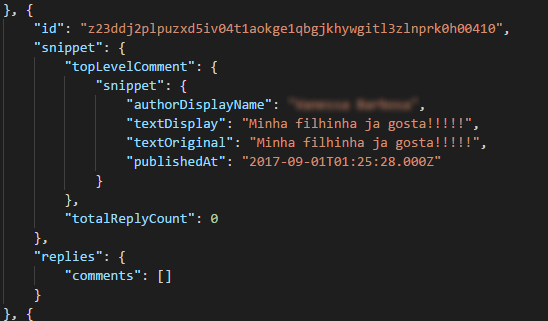
\includegraphics[scale=1]{figuras/figura_comentario_coletado.png} % altere o atributo scale para o tamanho da figura
	\end{center}
	\legend{Fonte: autor}
%Verificar se precisa por a data aqui 
\end{figure}


\subsection{Pré-Processamento}

Nesta etapa, um \textit{script} \footnote{https://gist.github.com/ssisaias/d6dd83361d6fa64c0341427b1f6f3f22} escrito em Python foi executado para extrair somente os textos dos comentários obtidos através da ferramenta de extração, o script também é capaz de remover caracteres que não são considerados, dentro do contexto desta pesquisa, como \textit{emojis}. 

Em seguida, através da ferramenta NLTK, o pré-processamento foi realizado de foram automática: os acentos foram removidos e os textos foram \textit{tokenizados}, através de um processo que remove palavras sem valor semântico para o classificador e reduz palavras com valor semântico ao seu radical, através dos métodos \textit{word\_tokenize()} e \textit{RSLPStemmer()} presentes na NTLK. Ao final dessa etapa, um arquivo contendo os comentários devidamente pré-processados é gerado. 

\subsection{Treinamento do Modelo de Classificação}
Em posse dos comentários pré-processados, foi obtido um modelo de classificação da seguinte forma:

Primeiramente, o dicionário da \textit{SentiStrength} deve estar previamente estabelecido, o autor obteve um dicionário pronto para a língua portuguesa já fornecido no site da ferramenta e o melhorou e adaptou para o contexto deste trabalho, removendo algumas palavras em inglês que estavam erroneamente no dicionário e adicionando os palavrões necessários para a classificação de comentários com termos pejorativos. Os palavrões adicionados podem ser encontrados no Apêndice B.

A versão do \textit{SentiStrength} utilizada foi a 2.3, específica para Sistemas Operacionais Windows. Através de sua interface gráfica, o arquivo foi gerado pelo \textit{script} \footnote{https://gist.github.com/ssisaias/d6dd83361d6fa64c0341427b1f6f3f22} da etapa de pré-processamento. Após a classificação gerada pelo \textit{SentiStrength}, alguns comentários foram verificados manualmente pelo autor, esse procedimento se refere à classificação assistida. Frases que foram classificadas como pejorativas erroneamente por possuírem, por exemplo, o seguinte \textit{emoticon} \textbf{:(}, foram reclassificadas como neutras, pelo próprio autor. Ou seja, não expressão sentimento pejorativo.

Outro \textit{script}\footnote{https://gist.github.com/ssisaias/08b2c8494a4553612987c9d4ae94f86c} é então executado para "\textbf{traduzir}" a classificação feita pela \textit{SentiStrength}. O funcionamento desse \textit{script} se dá do seguinte modo: Quando a classificação de um comentário é dada como positiva pela ferramenta, é então convertida para \textbf{0} (ou classificação neutra); Quando a classificação é negativa, espera-se que haja um termo pejorativo no comentário e esse é classificado com o valor \textbf{1}. Isso faz com que o modelo de classificação apenas se preocupe com as duas classes determinadas que são neutra e pejorativa.

De posse dos comentários que compõem o grupo de treino devidamente classificados, utilizou-se a biblioteca \textit{scikit-learn}, para criação do modelo de classificação. O procedimento está descrito a seguir. 

No trecho de código abaixo, as variáveis \textbf{counts} e \textbf{targets} representam a lista com os comentários e a lista com suas classificações, respectivamente. A variável \textbf{classifier} recebe a nova instância do classificador MultinomialNB, e que em seguida é "alimentada"\ com os dados dos comentários e sua classificação. O modelo de classificação é então criado.

\begin{lstlisting}[frame=single, language=Python]  % Start your code-block

from sklearn.naive_bayes import MultinomialNB 
classifier = MultinomialNB()
classifier.fit(counts,targets)

\end{lstlisting}


\subsection{Avaliação do Modelo de Classificação}

Nesta etapa, os comentários separados para o grupo de teste foram submetidos ao classificador. Também foram submetidos todos os outros comentários obtidos, tendo estes passado pelo mesmo procedimento de pré-processamento, classificação na ferramenta \textit{SentiStrength}, análise humana, e enfim, classificados pelo modelo gerado anteriormente.

A exemplo do grupo de testes mencionado na criação do modelo de classificação, uma matriz com os comentários é passada para o método \textbf{predict()} do classificador. A variável \textbf{predictions} contém a classificação gerada, que agora pode ser avaliada de acordo com os valores esperados.

\begin{lstlisting}[frame=single, language=Python]  
predictions = classifier.predict(teste_counts)
\end{lstlisting}

A avaliação do modelo é feita através da ferramenta Scikit Learn, que fornece métodos de \textit{score} prontos para as medidas de \textit{precision} e \textit{recall}. Um \textit{script} \footnote{https://gist.github.com/ssisaias/b9521c910d66c440c9e90d21f5360536} auxiliar foi criado com os passos de validação. Os resultados da avaliação são apresentados no próximo capítulo.



\subsection{Extensão do Google Chrome - SafeYoutube}

Após gerar e avaliar o modelo de classificação, e obter os resultados, foi desenvolvida uma extensão do navegador da web Google Chrome que se utiliza de um \textit{Web Service} que retorna a margem de comentários negativos e positivos para o vídeo sendo assistido naquele momento.

A extensão \textbf{SafeYoutube} foi criada utilizando as tecnologias web HTML, CSS e Javascript. Como referência para o desenvolvimento foi utilizada a documentação oficial para desenvolvedores Chrome \footnote{https://developer.chrome.com/extensions}. Sua arquitetura é descrita no diagrama da Figura \ref{fig:chrome_plugin_design}. Os códigos-fonte da extensão \footnote{https://github.com/ssisaias/safe-youtube} e do serviço web \footnote{https://github.com/ssisaias/safe-youtube-service}, estão disponíveis publicamente e podem ser encontrados na plataforma Github.

\begin{figure}[H] %use h para forçar que a figura fique abaixo do texto
	\caption{\label{fig:chrome_plugin_design} Arquitetura da extensão desenvolvida}
	\begin{center}
	    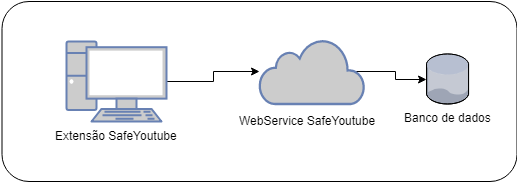
\includegraphics[scale=0.7]{figuras/safeYoutube.png} % altere o atributo scale para o tamanho da figura
	\end{center}
	\legend{Fonte: Autor}
%Verificar se precisa por a data aqui 
\end{figure}

Ao entrar um vídeo do youtube com a extensão \textbf{SafeYoutube} instalada, ela permite que o usuário a selecione, exibindo assim os resultados de uma classificação realizada previamente para aquele vídeo. Um exemplo do funcionamento é visto na Figura \ref{fig:chrome_plugin}. 

Caso os comentários do vídeo ainda não tenham sido classificados, o serviço irá iniciar um procedimento automático de classificação, tornando os resultados disponíveis dentro de um intervalo de tempo. O procedimento automático de classificação segue os mesmo procedimentos listados nas etapas de \textbf{pré-processamento} e \textbf{avaliação do modelo}, ou seja, os comentários são coletados, pré-processados, e classificados com o modelo de classificação gerado na etapa de \textbf{Treinamento do Modelo}.

\begin{figure}[H] %use h para forçar que a figura fique abaixo do texto
	\caption{\label{fig:chrome_plugin} Extensão SafeYoutube}
	\begin{center}
	    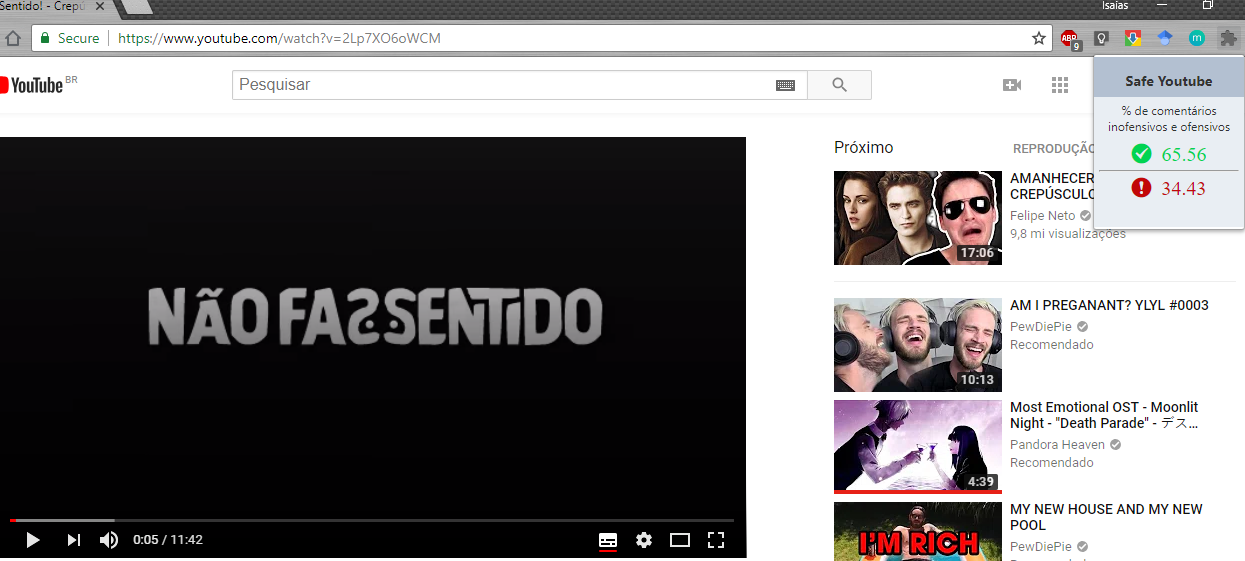
\includegraphics[scale=0.4]{figuras/extensao_chrome_normal.png} % altere o atributo scale para o tamanho da figura
	\end{center}
	\legend{Fonte: Autor}
%Verificar se precisa por a data aqui 
\end{figure}

\begin{figure}[H] %use h para forçar que a figura fique abaixo do texto
	\caption{\label{fig:chrome_plugin_zoom} Extensão SafeYoutube - Imagem ampliada}
	\begin{center}
	    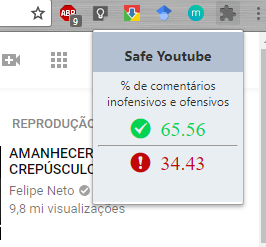
\includegraphics[scale=0.7]{figuras/extensao_chrome_zoom.png} % altere o atributo scale para o tamanho da figura
	\end{center}
	\legend{Fonte: Autor}
%Verificar se precisa por a data aqui 
\end{figure}

Nota-se pelo \textit{plugin} no canto superior direito da Figura \ref{fig:chrome_plugin_zoom}, que o vídeo em questão possui 65.56\% de comentários positivos e 34.43\% de comentários negativos.

